\lstset{language=C}
\section{Session 5}
\subsection{Constructing the mesh II}
\paragraph{}In the last session we worked with three different \texttt{.stl} files but we can also put all of these surfaces in a single file. To do so, we must modify the one of the files in order to append all he geometries. The Pdf \texttt{pipe.pdf} which can be found in atenea explains all the process.
\begin{enumerate}
	\item Put all the solids into a single file
	\item Modify SnappyHexMesh dictionary to specify these solids 	into the regions section.
\end{enumerate}
\paragraph{}The process is nearly the same as in the session 4. When executing a command we can print the terminal output of the command to a log (e.g \texttt{snappyHexMesh > snappy.log} or \texttt{foamJob snappyHexMesh, this one prints also the output to the terminal}. we can clean the polymesh folder directy by tipping \texttt{foamCleanPolyMesh}. If we want to only have a single mesh stored in the constant folder we can do it by tipping \texttt{snappyHexMesh -owerwrite} 

\subsection{Simulating the case}
\paragraph{}A good advice before simulating a case is to make a copy of the 0 folder in order to be able to reset the case.

\paragraph{}Now we are going to edit the \texttt{0} inside the 0.orig folder to put our boundary conditions. Inside the boundary section of this file we have to modify the code to appear as following.
inlet1 0 -1 0
inlet2 -10 0 0

\begin{lstlisting}
internalField uniform(0 0 0);

.... %delete all the include lines under initialConditions

patchName
{
	type		fixedValue;
	value 		uniform(Ux Uy Uz);
}
\end{lstlisting}
\paragraph{}the \texttt{inletOutlet;} option in the type field means that in the oultet when the flow is going out of the domain the boundary condition is Zero Gradient avoiding the flow to returning inside of the domain.



fixedValue 
change it to uniform(0 0 0)
\subsection{Constructing the mesh}
\paragraph{}We want to make the mesh using \textbf{ParaView}. We can also use directly \emph{Salome-Meca} to mesh the pipe but its mesher is not as good as the one we're going to use. First we have to create a case. A good option is to look for a similar tutorial case as a basis for our mesh (and of course similar to the case we want to run). For the Y-pipe problem we can start with the motorbike case. To do so, create a folder and name it as Ypipe, then copy inside it the folders contained in the motorbike case. It can be done in a terminal by typing:
\begin{scriptsize}
\begin{lstlisting}
	mkdir -p Ypipe
	cp -r /opt/openfoam4/tutorials/incompressible/simpleFoam/motorBike/* ./Ypipe
\end{lstlisting}
\end{scriptsize}

\paragraph{}Once we have the folder created the first we are going to do is to create a folder inside the constant folder containing the \texttt{.stl} files file. (Copy the .stl an paste it in /constant/trisurface and rename it as Ypipe). The next step is  go to the  \texttt{system} folder, inside there is a file named \texttt{BlockMeshDict}. We must modify the block geometry to put the pipe inside it. The new values for the vertices of the block are:
\begin{center}
\begin{lstlisting}
vertices
(
    (-1 -2.5 -0.5)
    (3 -2.5 -0.5)
    (3  3 -0.5)
    (-1  3 -0.5)
    (-1 -2.5 0.5)
    (3 -2.5 0.5)
    (3  3 0.5)
    (-1  3 0.5)
);
\end{lstlisting}
\end{center}
\paragraph{}We have to achieve a cells as regular as posible.
\begin{figure}[h!]
\centering
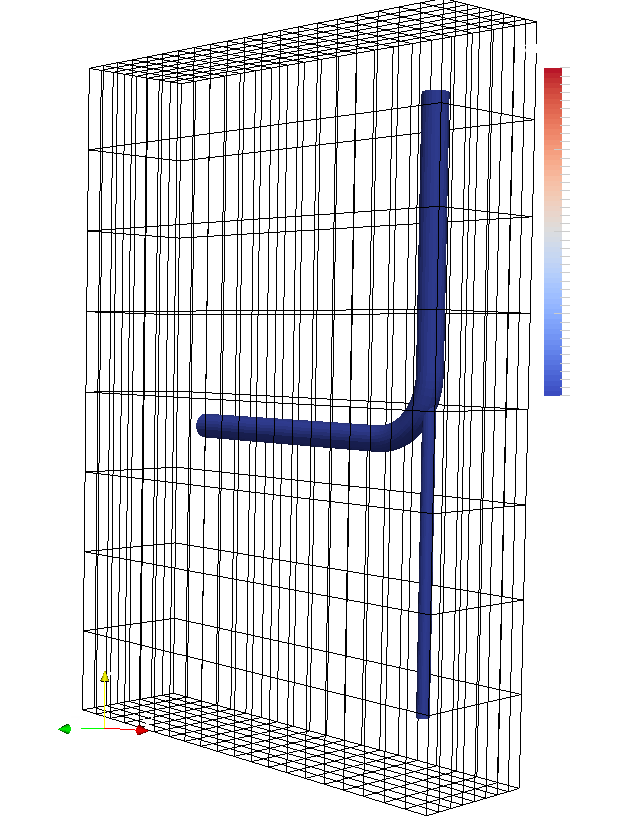
\includegraphics[scale=0.3]{mesh1.png}
\caption{First mesh. Toooooo coarse}
\end{figure}

\subsection{Refining the mesh}
\paragraph{}The next steps involve refining the mesh. To do so we are going to use \textbf{snappyHexMesh}(See reference). We must define the level 0 of the mesh. Open \texttt{BlockMeshDict} an edit the following lines:
\begin{center}
\begin{lstlisting}
blocks
(
    hex (0 1 2 3 4 5 6 7) (32 64 4) simpleGrading (1 1 1)
);
\end{lstlisting}
\end{center}

\paragraph{}The next step is to take \texttt{SnappyHexMesh} dictionary. Rather than create it is better to take it from \texttt{openfoam4/applications/uilities/mesh/generation/\\snappyhexmesh} and paste it to the \texttt{Ypipe/system} folder. Inside the file there are a lot of comments and explanations about the mesh configuration and parameters.

\paragraph{}It is possible to define an upper level of discretization inside our blockMesh using searchablebox

\paragraph{}\textbf{SnappyHexMesh} is one of the only meshers that can perform a parallel mesh of the domain (using multiple cores). The parameter \texttt{maxLocalCells} and \texttt{maxGlobalCells} define the maximum number of cells per core and the maximum number of cells on the global mesh respectively.



.......
.......
.......\\\\\\\\\


the parameter \texttt{LocationInMesh} let us decide wether we want to mesh inside or outside our geometry. the input has to be a point inside of the object

inside the folder \texttt{Ypipe/trisurface} we must have the four surfaces .stl files.